% begin module newtons-method-def
\begin{frame}
Goal: find a root $r$ of $f(x)$.
\begin{columns}[c]
\column{.45\textwidth}
\psset{xunit=1cm, yunit=1cm}
\begin{pspicture}(-5, -5)(5,5)
\psframe*[linecolor=white](-5,-5)(5,5)
\psaxes[ticks=none, labels=none]{<->}(0,0)(-0.5,-0.5)(4.5,4)\tiny
\fcLabels{4.5}{4}
%Function formula: (1/2 (x))^{2}-3/10
\rput[r](2.8,2){$y=f(x)$}
\psplot[linecolor=red, plotpoints=1000]{0}{4}{-0.3 x 0.5 mul 2 exp add }
\fcXTick{1.095445115}
\rput[b](1.095445115, 0.2){$r$}

\uncover<2->{\fcLabelOnXaxis{4}{\alertNoH{2}{$x_1$}}} %x_1:=4; f{}x_1:=3.7;
\uncover<3-5,10-16>{
\psline[linestyle=dashed](4,0)(4,3.7)
\fcFullDot{4}{3.7}
%Function formula: -43/10+2 (x)
\psplot[linecolor=\fcColorTangent, plotpoints=1000]{2}{4}{x 2 mul -4.3 add }
}

\uncover<4->{\fcLabelOnXaxis{2.15}{\alertNoH{4,16}{$x_2$}}} %x_2:=43/20; f{}x_2:=0.855625;

\uncover<6-7,17-23>{
\psline[linestyle=dashed](2.15,0)(2.15,0.855625)
\fcFullDot{2.15}{0.855625}
%Function formula: -2329/1600+43/40 (x)
\psplot[linecolor=\fcColorTangent, plotpoints=1000]{1.1}{4}{x 1.075 mul -1.45562 add }
}

\uncover<7->{\fcLabelOnXaxis{1.354069767}{\alertNoH{7,23}{$x_3$}}} %x_3:=1354069767/1000000000; f{}x_3:=0.158376;
\uncover<8>{
\psline[linestyle=dashed](1.354069767,0)(1.354069767,0.158376)
\fcFullDot{1.354069767}{0.158376}
%Function formula: -3033504933903434289/4000000000000000000+1354069767/2000000000 (x)
\psplot[linecolor=\fcColorTangent, plotpoints=1000]{0.7}{4}{x 0.677035 mul -0.758376 add }
}
\uncover<8->{
\fcLabelOnXaxis{1.120143514}{\alertNoH{8}{$x_4$}}
} %x_4:=1011168311301144763/902713178000000000

\end{pspicture}

%\ \only<handout:0| -2>{%
%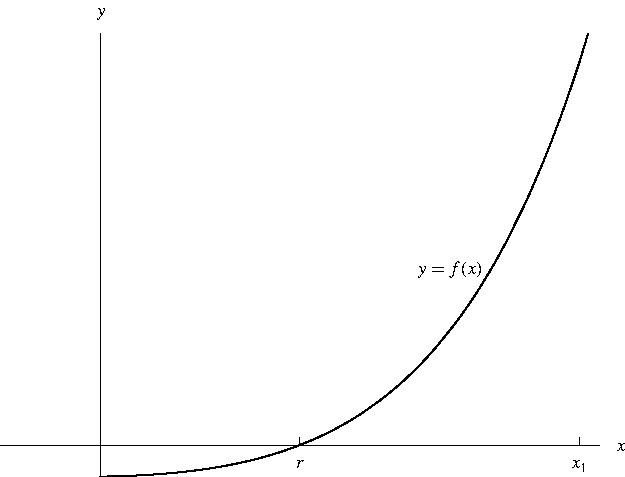
\includegraphics[height=4cm]{newtons-method/pictures/04-08-newtona.pdf}%
%}%
%\only<handout:0| 3-5,10-16>{%
%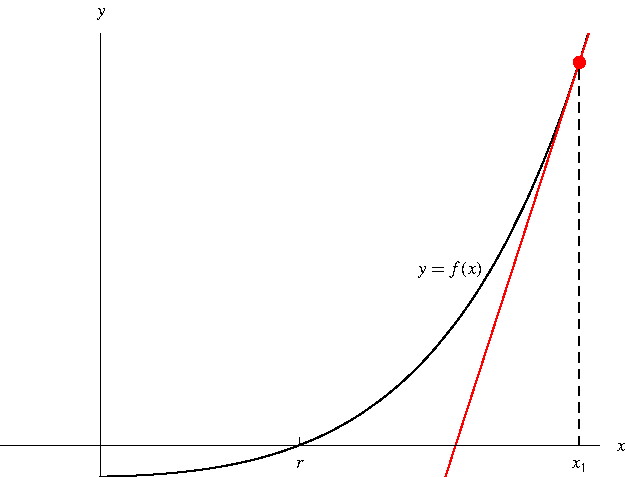
\includegraphics[height=4cm]{newtons-method/pictures/04-08-newtonb.pdf}%
%}%
%\only<handout:0| 6-7,17-22>{%
%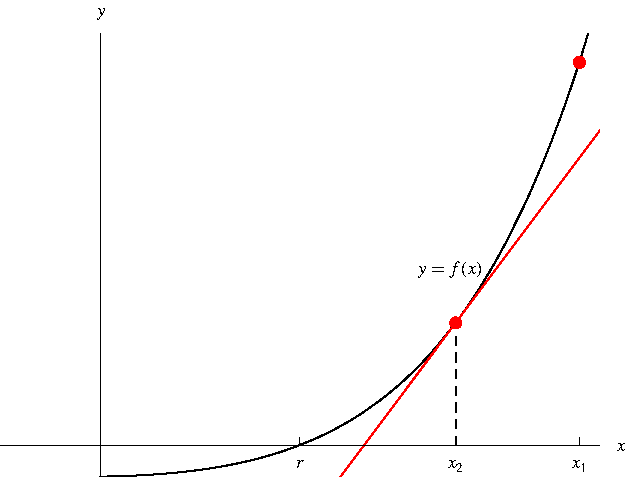
\includegraphics[height=4cm]{newtons-method/pictures/04-08-newtonc.pdf}%
%}%
%\only<handout:0| 8>{%
%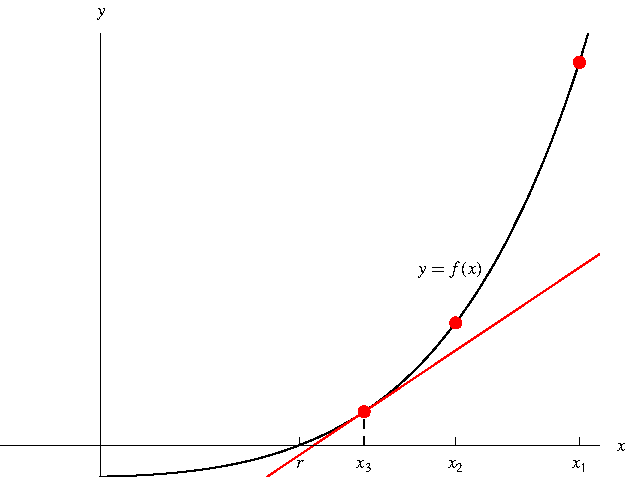
\includegraphics[height=4cm]{newtons-method/pictures/04-08-newtond.pdf}%
%}%
%\only<9,23->{%
%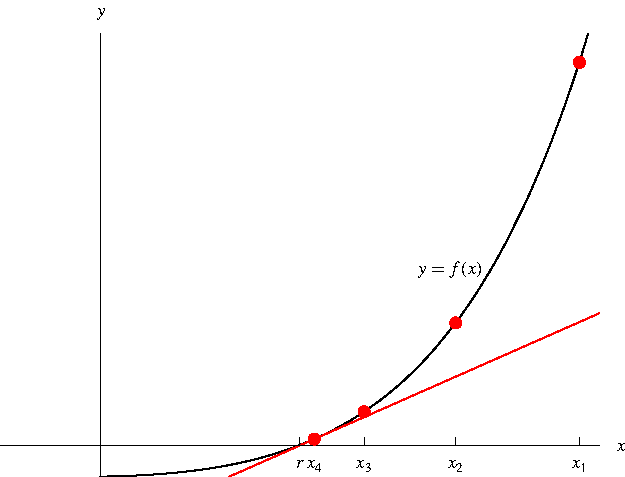
\includegraphics[height=4cm]{newtons-method/pictures/04-08-newtone.pdf}%
%}%

\column{.55\textwidth}

\begin{itemize}
\item<2->  Pick a number $x_1$.
\item<3-| alert@10-12>  Find the tangent to $f$ at $(x_1, f(x_1))$.
\item<4-| alert@13-15>  Call the $x$-intercept of this line $x_2$.
\item<5->  Repeat the process using $x_2$. %in the place of $x_1$:
\item<6-| alert@17-19>  Find the tangent to $f$ at $(x_2, f(x_2))$.
\item<7->  \alertNoH{20-23}{Call the $x$-intercept of this line $x_3$}, \uncover<8->{ \alertNoH{8,24}{and so on.}}
\end{itemize}
\end{columns}

\begin{columns}[c]
\column{.55\textwidth}
\abovedisplayskip=0pt
\belowdisplayskip=-15pt
\begin{align*}
\uncover<10-15,17-22>{\text{Equation:}}\quad
\uncover<10-15,17-22>{y - \uncover<12-15,19-22>{\alert<handout:0| 12,19>{f(x_{\only<handout:0| -15>{1}\only<handout:0| 16->{2}})}}} & \uncover<10-15,17-22>{=}  \uncover<11-15,18-22>{\alert<handout:0| 11,18>{f'(x_{\only<handout:0| -15>{1}\only<handout:0| 16->{2}})}}\uncover<10-15,17-22>{(x-\uncover<12-15,19-22>{\alert<handout:0| 12,19>{x_{\only<handout:0| -15>{1}\only<handout:0| 16->{2}}}})}\\
\uncover<13-15,20-22>{\text{$x$-intercept:}}\quad
\uncover<13-15,20-22>{\alert<handout:0| 13,20>{0} - f(x_{\only<handout:0| -15>{1}\only<handout:0| 16->{2}})} & \uncover<13-15,20-22>{=}  \uncover<13-15,20-22>{f'(x_{\only<handout:0| -15>{1}\only<handout:0| 16->{2}})(\alert<handout:0| 13,20>{x_{\only<handout:0| -15>{2}\only<handout:0| 16->{3}}}-x_{\only<handout:0| -15>{1}\only<handout:0| 16->{2}})}\\
\uncover<14-15,21-22>{f'(x_{\only<handout:0| -15>{1}\only<handout:0| 16->{2}})x_{\only<handout:0| -15>{1}\only<handout:0| 16->{2}} - f(x_{\only<handout:0| -15>{1}\only<handout:0| 16->{2}})} & \uncover<14-15,21-22>{=}  \uncover<14-15,21-22>{f'(x_{\only<handout:0| -15>{1}\only<handout:0| 16->{2}})x_{\only<handout:0| -15>{2}\only<handout:0| 16->{3}}}\\
\uncover<15,22>{x_{\only<handout:0| -15>{2}\only<handout:0| 16->{3}}} & \uncover<15,22>{=}  \uncover<15,22>{x_{\only<handout:0| -15>{1}\only<handout:0| 16->{2}} - \frac{f(x_{\only<handout:0| -15>{1}\only<handout:0| 16->{2}})}{f'(x_{\only<handout:0| -15>{1}\only<handout:0| 16->{2}})}}
\end{align*}
\column{.45\textwidth}
\[
\uncover<16->{\alertNoH{16}{
x_2 = x_1 - \frac{f(x_1)}{f'(x_1)}%
}}%
\]
\[
\uncover<23->{\alertNoH{23}{
x_3 = x_2 - \frac{f(x_2)}{f'(x_2)}%
}}%
\]
\[
\uncover<24,25->{\alertNoH{24}{
x_{n+1} = x_n - \frac{f(x_n)}{f'(x_n)}%
}}%
\]
\end{columns}
\end{frame}
% end module newtons-method-def
